\section{Daten} \label{Kapitel: Daten}
Die Aufnahmen wurden mit dem Highspeed-Kamera-Teststand (Abb.: \ref{HTA}) der Firma LaVision gemacht. \\
Dazu wurde DaVis (Kap.:\ref{DaVis}) benutzt, um circa 60.000 Aufnahmen von der Sieben-Segment-Anzeige zu machen.\\
\begin{figure}[h]
\centering
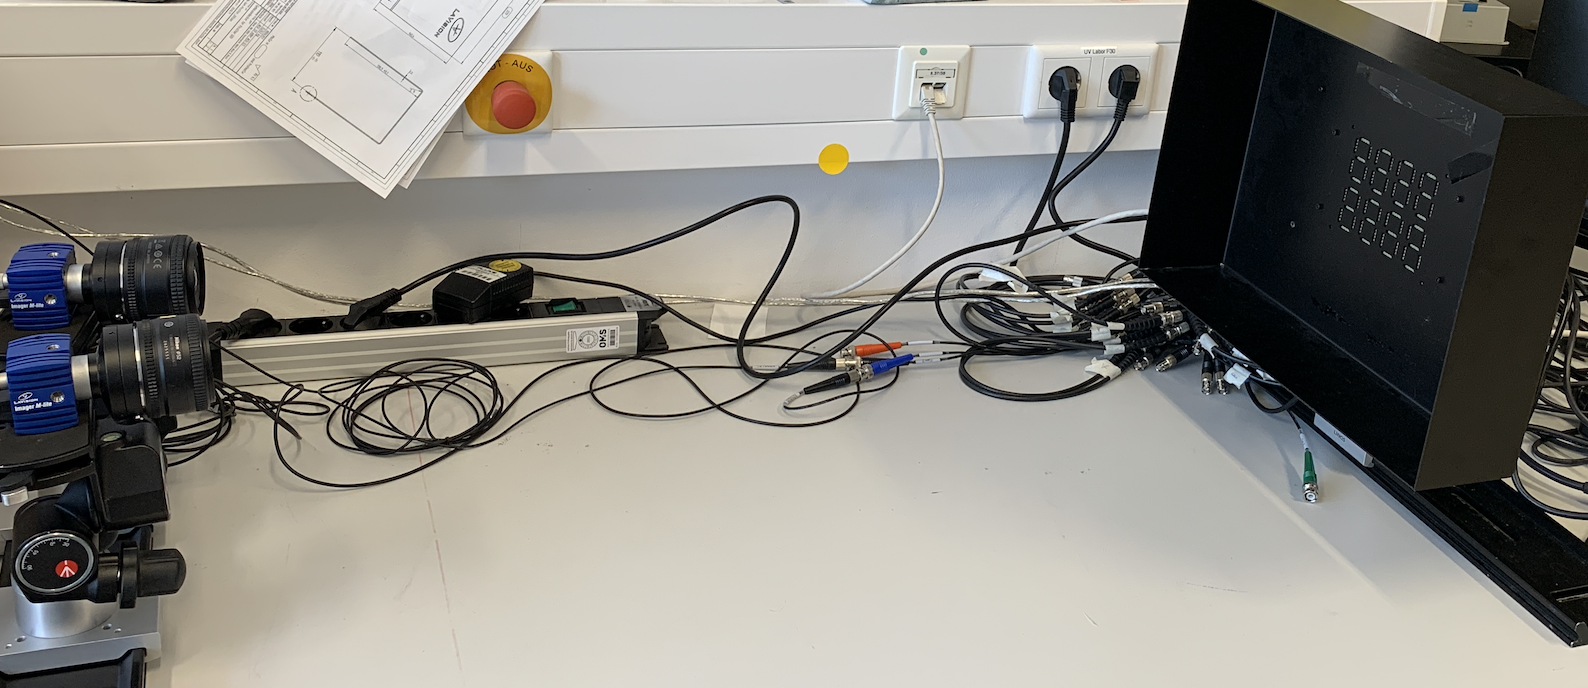
\includegraphics[scale=0.5]{pic/HTA}
\caption{Highspeed-Kamera-Teststand}
\label{HTA}
\end{figure}
Es wurde sich bei der Anzahl der Aufnahmen an dem MNIST \ref{MNIST} Datensatz orientiert. Es gibt keine genaue Methode, die Menge der nötigen Daten für das Maschinelle Lernen zu bestimmen, deswegen wird sich oft an schon vorhanden Beispielen orientiert. Eine andere Variante ist eine repräsentativitätsheuristische Methode, dabei wird versucht abzuschätzen, wie viele Beispiele ein Klasse braucht und dann diese Zahl mit der Anzahl der Klassen multipliziert. Als Beispiel in dieser Arbeit: Zehn Klassen mit zehn verschieden Einstellungen \`{a}  1.000 Aufnahmen wären insgesamt 100.000 Aufnahmen.
\subsection{Aufnahmen}
Bei den Aufnahmen wurde versucht, möglichst viele Parameter der Aufnahme zu verändern.  Bei der Veränderung der Parameter geht es darum,  möglichst viel Varianz in die Aufnahmen zu bringen. Einzig der Kameratyp und das Objektiv  (Kamera M-Lite 5M mit 35mm Objektiv) wurden nicht verändert.\\
Die Parameter, welche verändert wurden:
\begin{description} \label{Parameter}
\item[Belichtungszeit:] zwischen 88 $\mu$s und 1000$\mu$s in vier Schritten
\item[Lichtverhältnisse:] abgedunkelt, Deckenlicht und Deckenlicht mit Tageslicht
\item[Blende:] zwischen vier und 22 in fünf Schritten
\item[Abstand:]zwischen 77 cm bis 83 cm in drei cm Schritten
\item[Neigung:] die Kamera wurde zwischen -30\textdegree und +30 \textdegree in sieben Schritten gedreht
\item[Blickwinkel:] die Kamera hat zwischen einen Winkel von -20\textdegree und +20\textdegree in fünf Schritten auf die Anzeige geschaut
\end{description}
Aus den Bilder wurde dann mit DaVis (Kap.:\ref{DaVis}) das obere rechte Sieben-Segment ausgeschnitten.  Dieses ist die Ziffer,  die sich bei jeder Aufnahme ändert.  Die Aufnahme hat nun eine Größe von  712 $\times$ 82 Pixeln.\\
\\
\begin{tabular}{c | c}
\centering
\textbf{Ziffer} & \textbf{Anzahl der Aufnahmen} \\ \hline
Null & 5976\\
Eins & 5976\\
Zwei & 5976\\
Drei & 5976\\
Vier & 5976\\
Fünf & 5976\\
Sechs & 5977\\
Sieben & 5976\\
Acht & 5976\\
Neun & 5976\\
\end{tabular}\\
\\
Die Ziffern sind ausgesprochen gleich verteilt in dem Datensatz.
\subsection{Bearbeitung}
Zunächst wurde bei den Daten  visuell überprüft,  ob die Ziffern  noch in der Aufnahme sind und die Ziffern unterschiedlich genug sind.  Danach wurden eine Ziffer aus den Aufnahmen ausgeschnitten mit Hilfe  einer Maskenfunktion in DaVis  (Kap.:\ref{DaVis}).\\
Die gespeicherten Aufnahmen einer Ziffer wurde dann mit dem lvreader  (Kap.:\ref{lvreader}) in Python eingelesen und weiter bearbeitet.\\
Zuerst wurde alle Daten mit einer Zielvariablen (Label) versehen, dazu wurde die   Aufnahmesets beschriftet mit der ersten Ziffer,  die in dem Set zu sehen ist.  Die  Ziffern in einem Set laufen dann mit jeder Aufnahme eine Nummer (1,2,3...) weiter.\\
\lstinputlisting[language=Python,  firstline=8, lastline=21]{code/DataCreation.py}
Zur Reduzierung der Datengröße wurden die Aufnahmen auf ein Viertel der Originalgröße (zu 112 $\times$ 83 Pixeln) minimiert und zur besseren Darstellung invertiert.  Außerdem wurden sie in ein eindimensionales Array formatiert, so können sie direkt als Eingabewerte für ein Neuronales Netzwerk benutzt werden.\\
Zum Schluss wurden die Aufnahmen mit ihrem Label als numpy-Array gespeichert.\\
\lstinputlisting[language=Python,  firstline=62, lastline=67]{code/DataCreation.py}
\newpage
\begin{figure}[H]
\centering
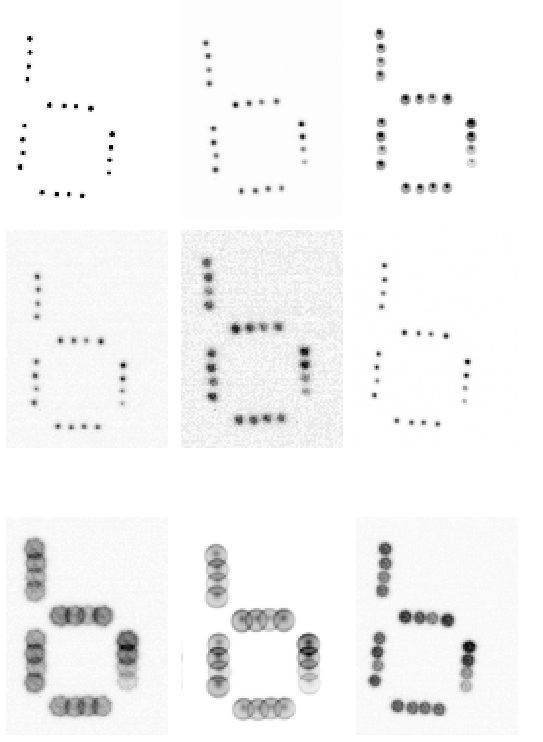
\includegraphics[scale=0.8]{pic/6Beispiel}
\caption{Beispiel der bearbeiten Aufnahmen} 
\end{figure}
\newpage
\subsection{Datenformat}
Das Datenformat npy wurde gewählt, da es sich leicht und nativ in TensorFlow weiterverarbeiten lässt.  Außerdem haben npy-Dateien eine schnellere Lesezeit und komprimieren die Daten besser als z.B. csv-Dateien. Beides ist hilfreich bei großen Datensätzen, wie sie für Maschinelles Lernen benötigt werden.\cite{url:npyFile-20210908}\\
\begin{figure}[h]
\centering
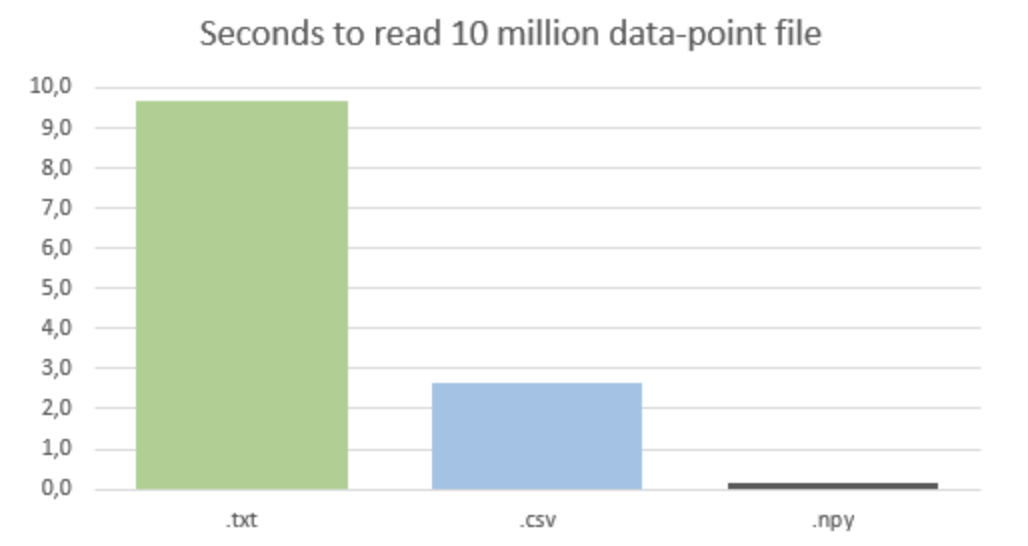
\includegraphics[scale=0.8]{pic/npyFile}
\caption{Lesegeschwindigkeiten der Datenformate \cite{url:npyFile-20210908}} \label{Lesegeschwindigkeiten}
\end{figure}

\subsubsection{Datenteilung}
Die Aufnahmen wurden in drei Datensätze unterteilt (Training-, Test- und Validierungssatz). Die Daten wurden vor der Unterteilung gemischt.  Die Unterteilung der Daten geschieht, damit nicht mit dem gleichen Datensatz getestet wie gelernt wird. Damit lässt sich erkennen, ob der Algorithmus nicht-besondere nicht-relevante Eigenschaft erlernt hat. \\
Der dritte Datensatz dient zur Validierung. Nachdem ein Modell mit dem Trainieren abgeschlossen hat, kann nun an dem Validierungssatz getestet werden, wie gut das Modell mit ihm unbekannte Daten umgeht.  Außerdem kann man unterschiedliche Modelle auf ihre Effizienz mit einander vergleichen.\\
Damit ein Vergleich der unterschiedlichen Modelle möglich war, wurden die gemischten und dann getrennten Datensätze abgespeichert. Die neue abgespeicherten Datensätze wurden für das Lernen benutzt.
